\chapter{Evaluation des Trainings durch Probanden}
Die Evaluation soll die Ergebnisse des Trainings zeigen. Außerdem soll das Umfeld für die Probanden erläutert werden und was die Aufgabe der Probanden ist.

\section{Umgebung zur Erkennung von Interaktionen}
Der Prototyp wird auf einem Sofa aufgebaut, welches für drei Personen ausgelegt ist. Jede zusammengesetzte Komponte aus Sensoren angebaut am ESP32 steht für einen Platz auf dem Sofa. Zwei ESPs haben einen FSR mehr, da diese an den äußeren Sitzplätzen mit einer Armlehne sind. Für den Prototypen ist es nicht wichtig, in welchem Raum, welche Möbel zusätzlich und welche Geräte im Raum sind.

\begin{figure}[H]
	\centering
		%[natürliche Breite in Pixeln, natürliche Höhe in Pixeln, Abhängigkeit von der Textbreite]
		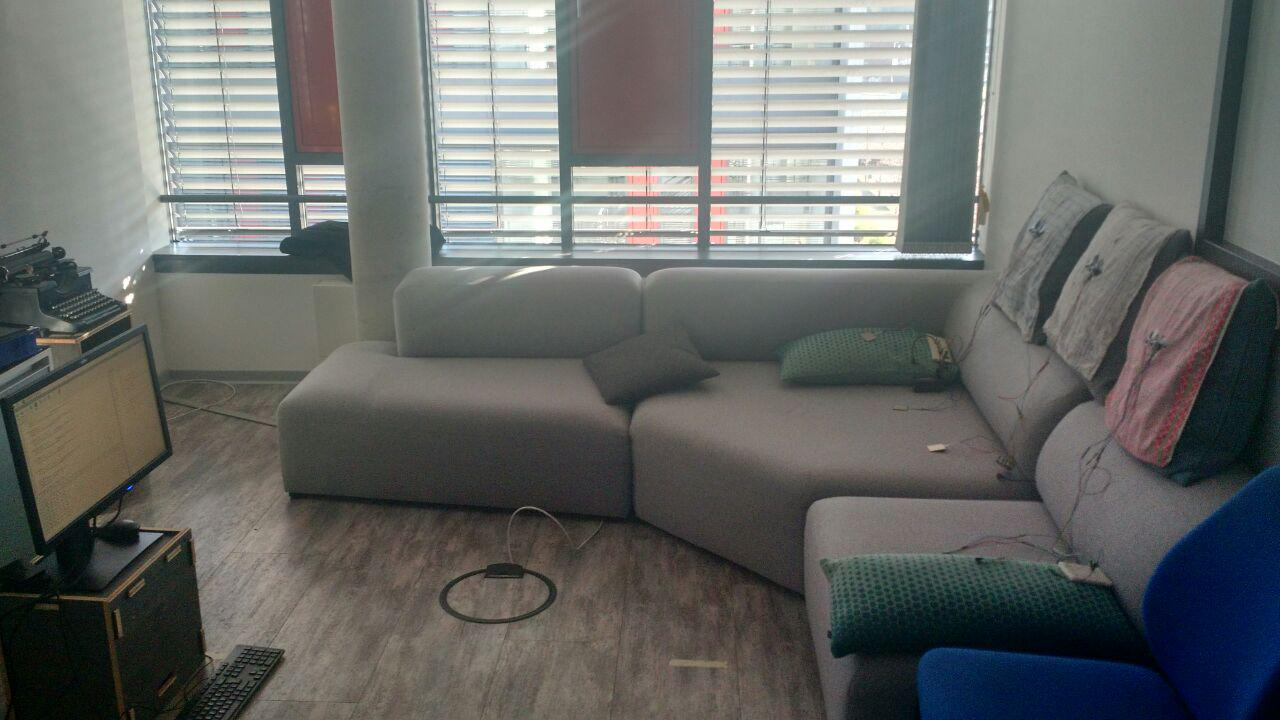
\includegraphics[width=0.75\textwidth]{images/prototyp.jpg}
	\caption{Realer Aufbau des Prototyps}
	\label{fig:prot}
\end{figure}

Abbildung \ref{fig:prot} zeigt den Prototypen, welcher auf einem Sofa platziert ist. Die beiden grünen äußeren Kissen stellen die Armlehnen dar. Da der Prototyp für ein drei Personen Sofa ausgelegt ist, werden die Sitzplätze durch die drei oben liegenden getrennt. Auf der linken Seite ist der Raspberry Pi mit dem MQTT Broker zu finden. Die Abbildung macht sichtbar, dass die Verwendung von Ultrasonic Sonic Sensoren nicht positiv ist. Man kann damit also zum Schluss kommen, dass statt Ultrasonic Sensoren - flachere Sensoren die weniger auffallen - eingebaut werden müssen.

\section{Ablauf der Situation}
\label{sec:abl}
Dieses Kapitel befasst sich mit der Beschreibung eines Ablaufs zur Sammlung der Daten über die Nutzung von Sensoren. Die folgende Beschreibung der Vorgehensweise zeigt auf, wie ein Proband in der Theorie mit dem Sofa interagieren soll um die bestmögliche Erfassung der Sensordaten zu bekommen.
\newline
\newline
Um die Klassifizierung richtig vorhersehen zu können, erstellen Probanden durch Interaktionen mit Sofa einen Trainingsdatensatz. Ein Proband befindet sich immer alleine im Raum mit dem Sofa. So kann kein anderer Proband durch seine Interaktionen beeinflusst werden. Dort nimmt er verschiedene Positionen auf dem Sofa ein. Hat dieser seine Position festgelegt werden die Sensorwerte in die CSV-Datei hinzugefügt. Die Position muss immer eine andere sein, damit die Variation mit den Sensoren sich so oft wie möglich unterscheidet. Der Proband soll sich also immer hinlegen, hinsetzen oder das Sofa leer lassen. Der Ablauf ist mit jedem Probanden gleich und unterscheidet sich nur von den Interaktionen auf dem Sofa. Sobald 12 bis 15 Probanden diese Situation absolviert haben, wird das neuronale Netz mit diesem Datensatz trainiert.

\subsection{Tatsächlicher Realablauf aller Probanden}
\label{sub:real}
Der Autor führt aus Kapitel \ref{sec:abl} an, wie eine Datensammlung in der Theorie mit einem Probanden ablaufen sollte. Der tatsächliche Ablauf mit allen Probanden erweist sich aber als differenz zur Theorie. Insgesamt wurden mit 17 Probanden Daten gesammelt. Die Anzahl der eingenommenen Positionen variiert, da verschiedene Interaktionen mehrfach auftreten. Je mehr Probanden mit dem Sofa interagieren, desto häufiger treten damit die gleichen Positionen auf.

\section{Aufbau des Datensatzes}
Hier soll gezeigt werden, wie die Sensordaten für die Trainings- und Testphase gespeichert werden. Eine Position des Probanden ist eine Liste die als eine Zeile in einer CSV-Datei liegt. Eine weitere CSV-Datei enthält die Outputs, die dem neuronalen Netz als Input ausgeben, welche Position die aktuelle Zeile aus der CSV-Datei zeigt. Kapitel \ref{cha:eval_NN} diskutiert die Ergebnisse aus dem neuronalen Netz und welche Optimierungen im weiteren vorgenommen werden, damit die Vorhersagen mit den Testdaten genauer sind.

\begin{table}[ht]
	\centering
	\caption[Aufbau eines Arrays des Datensatzes]{Aufbau eines Arrays des Datensatzes}
		\vspace{1.0em}	
	\begin{tabular}{| l | p{5cm} | l | }
		\hline
		\rowcolor[gray]{0.9}\textbf{Sensor} & \textbf{Beschreibung} & \textbf{Werte} \\
		\hline
		\hline
		Sitzkissen links &  & 0 bis maximal 4095\\
		\hline
		Armlehne links & & 0 bis maximal 4095\\
		\hline
		Rückenlehne links & & ca. 3000 bis maximal 0 \\
		\hline
		Sitzkissen mitte & & 0 bis maximal 4095\\
		\hline
		Rückenlehne mitte & & ca. 3000 bis maximal 0\\
		\hline
		Sitzkissen rechts & & 0 bis maximal 4095\\
		\hline
		Armlehne rechts & & 0 bis maximal 4095\\
		\hline
		Rückenlehne rechts & & ca. 3000 bis maximal 0\\ 
		\hline
	\end{tabular}
	\label{tab:tableqos}
\end{table}

\subsection{Ergebnisse der Datensammlung}
Es lässt sich anhand der Ergebnisse aus der Datensammlung zeigen, dass die FSR Sensoren auch Werte größer null ausgeben, obwohl die Probanden keinen Druck auf diese ausüben. Daraus lässt sich schlussfolgernd ziehen, dass das neuronale Netz auch diese Ausreißer erkennen muss. Damit bezweckt man, die trotzdem positiven Ergebnisse aus der Vorhersage zur Erkennung der Interaktionen. Weiterhin sei auch zu erwähnen, dass die Abstandserkennung durch die Ultrasonic Sensoren bei geringen Abständen sehr genau arbeitet. Wenn sich ein Proband anlehnt, kann es auch vorkommen, dass ein Kabel von einem Ultrasonic Sensor entfernt wird. Tritt dieser Fall auf, wird in der Datensammlung der Wert null gespeichert. Mit diesen Ergebnissen steht es außer Zweifel, dass die Datensammlung für das neuronale Netz geeignet ist. 

\section{Erkenntnisse aus der Evaluation}
Aus folgender Überlegung aus dem Kapitel \ref{sub:real}, dass Probanden nach einer Zeit wiederholt die gleiche Sitzposition einnehmen, werden in diesem Kapitel die Schlüsse und Erkenntnisse daraus gezogen.
So deuten diese Ergebnisse darauf hin, dass es von Vorteil ist, mehr Sensoren zur Erkennung der Interaktionen auf dem Sofa zu verbauen. Als weitere Möglichkeit geht daraus hervor, entweder nur FSR Sensoren zu verwenden und für die Sitzfläche Sensoren zu verbauen, welche die komplette Fläche einnehmen.

\section{Evaluation des neuronalen Netzes}
\label{cha:eval_NN}
